\documentclass{article}
\usepackage[utf8]{inputenc}

\title{Kuiper Belt Orbital Period}
\author{Skylar Liang }
\date{March 14,2020}

\usepackage{natbib}
\usepackage{graphicx}

\begin{document}

\maketitle

\section{About Kuiper Belt}
Kuiper Belt is a region of space outside our very outer planet in the Solar System, Neptune. It starts from the orbit of Neptune and contains with the icy object. Itself and the Oort Cloud are considered to be the source of comets\citep{kuiper}. Most likely, the icy objects are the leftover of the form of our Solar System. \\
More interestingly, Pluto was actually the first object discovered in the Kuiper Belt in 1930\citep{kuiper}. \\
For PI day, I'm going to make a rough calculation of the orbital period of this interesting region by calculating the orbital period of one of its objects that has the characteristics to represent the entire region, which will give me a estimated answer of the region's orbital period.

\begin{figure}[h!]
\centering
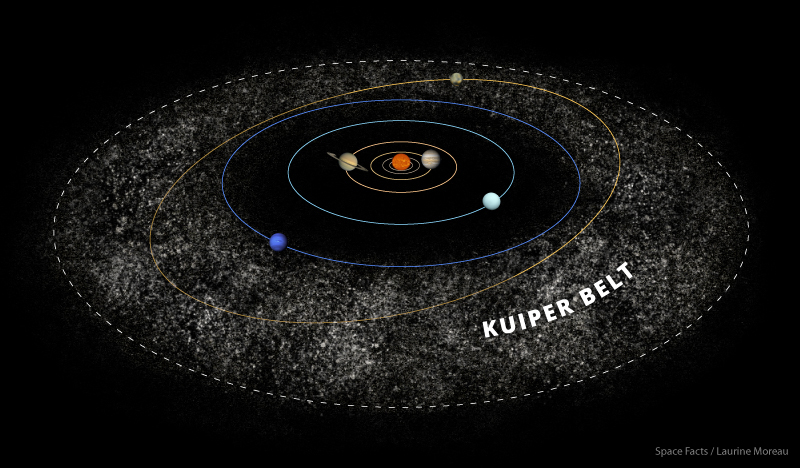
\includegraphics[scale=0.4]{kuiper-belt.png}
\caption{The Kuiper Belt}
\label{fig:kuiper-belt}
\end{figure}

\section{Calculation of the Orbital Period}
\subsection{Mean-Motion Resonance}
In fact, the orbital period of Kuiper Belt is the exact ratio of Neptune's, which is called mean-motion resonance. The Kuiper Belt orbits the Sun twice for every three Neptune orbits\citep{resonance}, which makes it $2:3$ ratio to the orbital period of Neptune. Since the Neptune orbits the sun every 165 years, we can roughly calculate the orbital period of Kuiper Belt to be every 247.5 years.
\subsection{Calculation Using $\pi$}
We cannot directly calculate the orbital period of a disk shaped region, however, the spacecraft New Horizons picked up a the Kuiper Belt object 2014 MU69. Recently, it has been officially named Arrokoth, a Native American term meaning “sky” in the Powhatan/Algonquian language\citep{sky}. \\
We know that Arrokoth is about $6.6\times 10^{9}$ km away from the Earth, which is almost the average of the inner and outer oundary of the Kuiper Belt. And, it has a orbit that is almost a perfect circle with a inclination of $2.4$ degree, which is a great representative of the disk region.
\begin{itemize}
    \item By using the formula for the circumference of a circle, we can calculate the distance of one period.\\
    \begin{equation}
        C = 2\pi r
    \end{equation}
    Distance from the sun:\\
    $C = 2\pi (6.6\times 10^{9}$ km $+ 1.5\times 10^{8}$ km $)$ \\
    $C = 2\pi (6.75\times 10^{9}$ km $) \approx 42411500823$ km
    \item Change the unit of the radius to meter, and then calculate the velocity.\\
    \begin{equation}
        V = \sqrt{\frac{GM_{Sun}}{r}}
    \end{equation}
    $V = \sqrt{\frac{(6.67\times 10^{-11}m^{3}kg^{-1}s^{-2})\cdot (2\times 10^{30}kg)}{6.75\times 10^{12}m}}$\\
    $V \approx 4446$ m/s
    \item Change the unit of circumference to meter, calculate the period in seconds.\\
    \begin{equation}
        t = \frac{C}{V}
    \end{equation}
    $t = \frac{42411500823000m}{4446 m/s} \approx 9539248948$s
    \item Change the unit of the period to years.\\
    $(9539248948s) \cdot \frac{1 min}{60s} \cdot \frac{1 hour}{60 min} \cdot \frac{1 day}{24 hours}\cdot \frac{1 year}{365 days} \approx 300 $ years
\end{itemize}

\section{Conclusion}
Comparing to the actual orbital period of the Kuiper Belt, which is 200 years, this calculation is not too far away from it consider the way of estimation. However, compare to the actual orbital peroid of Arrokoth, which is 297 years, this calculation is very close to the actual number of years. 

\bibliographystyle{plain}
\bibliography{references}
\end{document}
